\chapter{Recurrent Neural Networks}

Recurrent Neural Networks (RNN) can be used in a wide variety of tasks as they can work with inputs and outputs of variable size as shown in Figure \ref{rnn-applications}.
\begin{figure}[H]
    \centering
    \includegraphics[width=\textwidth]{Images/rnn.jpeg}
    \caption{The applications of Recurrent Neural Networks \cite{unres-rnn}}
    \label{rnn-applications}
\end{figure}

\begin{enumerate}
     \itemsep0em
     \item \textbf{One to one}: A vanilla neural network with fixed-sized input and fixed-sized output.
     \item \textbf{One to many}: An RNN with sequence output, e.g. image captioning: generate a sentence describing an input image.
     \item \textbf{Many to one}: An RNN with sequence input, e.g. sentiment analysis: infer the emotion of a given sentence.
     \item \textbf{Many to many (1)}: Sequence input and sequence output, e.g.: machine translation: output a sentence in Spanish given a sentence in English.
     \item \textbf{Many to many (2)}: Synced sequence input and output, e.g.: video classification: label each frame of a video.
\end{enumerate}

%%%%%%%%%%%%%%%%%%%%%%%%%%%%%%%%%%%%%%%%%%%%%%%%%%%%%%%%%%%%
%%%%%%%%%%%%%%%%%%%%  NEW SECTION   %%%%%%%%%%%%%%%%%%%%%%%%
%%%%%%%%%%%%%%%%%%%%%%%%%%%%%%%%%%%%%%%%%%%%%%%%%%%%%%%%%%%%
\section{Vanilla RNN}
Traditional neural networks do not have any memory as each input of the network are independent. Recurrent neural networks use loops to make information persist:

\begin{figure}[H]
    \centering
    \includegraphics[width=0.3\textwidth]{Images/vanilla-rnn.png}
    \caption{A vanilla recurrent neural network \cite{colah}}
    \label{vanilla-rnn}
\end{figure}

Given an input $x_t$ and a layer $A$, the output $h_t$ is fed again to $A$ during the next step along with the next input $x_{t+1}$. This becomes clearer when we unroll the RNN:

\begin{figure}[H]
    \centering
    \includegraphics[width=\textwidth]{Images/vanilla-rnn2.png}
    \caption{An unrolled vanilla recurrent neural network \cite{colah}}
    \label{unrolled}
\end{figure}

Basically, if we denote the function of layer A by $f$:
\begin{equation}
    h_t = f(h_{t-1}, x_t)
\end{equation}

Suppose the input $x_t \in \mathbb{R}^{D}$ and the layer $A$ contains $H$ neurons. Denote $W_x \in \mathbb{R}^{D\times H}$ the weights of the input, and $W_h \in \mathbb{R}^{H\times H}$ the weights of the hidden state. Then the explicit expression of $f$ is simply:
\begin{equation}
    h_t = \text{tanh}(W_x^T x_t + W_h^T h_{t-1})
\end{equation}

With $t \in \mathbb{N}^*$ and $h_0$ a randomly initialised vector. The expression of $h_t$ is similar to the neurons in a traditional neural network with a tanh (hyperbolic tangent, see Figure \ref{tanh}) activation function and two inputs instead of one.

\begin{figure}[H]
    \centering
    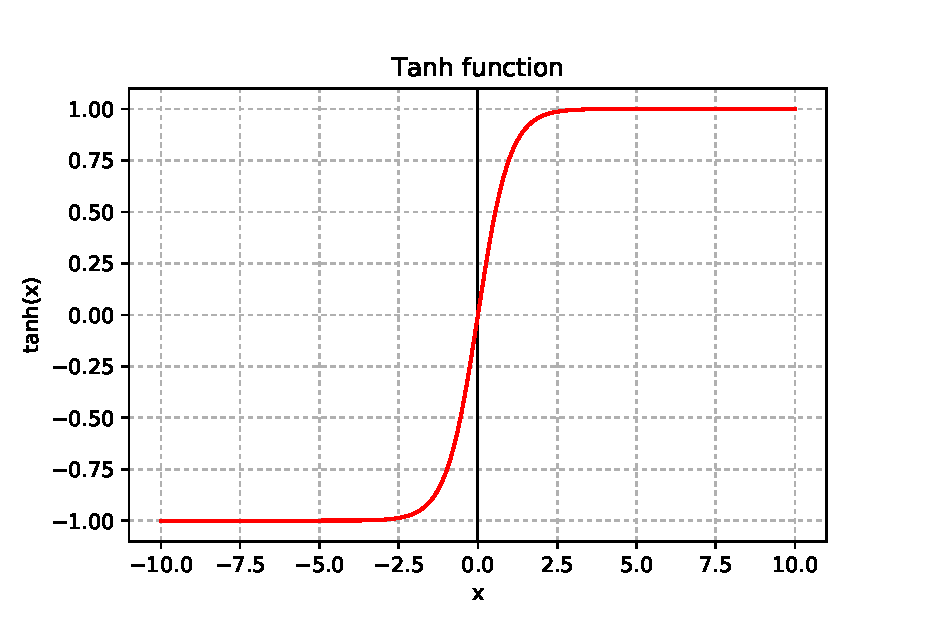
\includegraphics[width=0.5\textwidth]{Images/tanh.eps}
    \caption{Another activation function: tanh}
    \label{tanh}
\end{figure}

The vanilla RNN is a good progress towards learning from sequential inputs but is actually difficult to train as we'll see shortly.

\section{On the Difficulty of Training Vanilla RNNs}
In order to train a recurrent neural network, we unroll the network for $T$ steps (chosen depending on what kind of dependency we want to learn and also on memory limitation) then backpropagate through the unrolled network.

Concretely, if we ignore the inputs $x_t$ and consider that $h_t = \text{tanh}(a_t)$ with $a_t = W_h^T h_{t-1}$, the gradients of the hidden states are computed as: for t=1..T:
\begin{itemize}
    \item $\frac{\partial L}{\partial a_t} = 1 - \text{tanh}^2(\frac{\partial L}{\partial h_t})$
    \item $\frac{\partial L}{\partial h_{t-1}} = W_h \frac{\partial L}{\partial a_t}$
\end{itemize}

Note that we also ignored the gradient coming through the output neurons and basically only backpropagated through the the green neurons in Figure \ref{unrolled}. Now suppose that $W_h$ is a scalar, then as the gradient $\frac{\partial L}{\partial h_{t-1}}$ is repeatedly multiplied by $W_h$, if $W_h > 1$ the gradient diverge and if $W_h < 1$ the gradient goes to zero. Similarly in the general case $W_h \in \mathbb{R}^{H\times H}$, let us denote by $\lambda_{\text{max}}$ the largest eigenvalue of $W_h$ then Pascanu et al. proved in \cite{difficulty-rnn} that:

\begin{itemize}
    \item If $\lambda_{\text{max}} > 1$, the gradients will explode.
    \item If $\lambda_{\text{max}} < 1$, the gradients will vanish.
\end{itemize}

To prevent the gradients from exploding, Pascanu et al. proposed gradient clipping: if the norm of the gradient exceeds a threshold, then simply clip the gradient. If we denote by $g$ the gradient, then more formally, if $\Vert g \Vert > \text{threshold}$, then set $g$ to $\frac{\text{threshold}}{\Vert g \Vert} g$.

To address the vanishing gradient problem in recurrent neural networks, we use a variant of Vanilla RNN called Long-Short Term Memory (LSTM) \cite{lstm} that does not have vanishing gradients.

\section{Long Short-Term Memory}
The vanilla RNN is hard to train as the gradients often either vanish or explode. LSTMs solve this problem by using a gating mechanism. 

They keep track of the hidden state vector $h_t \in \mathbb{R}^H$ but also of a cell state vector $c_t\in \mathbb{R}^H$, we'll shortly explain. First, we compute the activation vector $a \in \mathbb{R}^{4H}$ that is 4 times bigger than vanilla RNN, which is necessary to remember long and short-term features. 
\begin{equation}
a = W_x^T x + W_h^T h
\end{equation}
with $x \in \mathbb{R}^{D}$, the input, $h \in \mathbb{R}^{H}$, the hidden state, $W_x \in \mathbb{R}^{D\times 4H}$ and $W_h \in \mathbb{R}^{H\times 4H}$.

Then this activation vector $a$ is split into 4 vectors: $a_i, a_f, a_o, a_g \in \mathbb{R}^H$, where $a_i$ is made up of the first $H$ elements of $a$, $a_f$ the $H$ next, etc. The so-called {\em gates}: the input gate $i \in \mathbb{R}^H$, the forget gate $f \in \mathbb{R}^H$, the output gate $o \in \mathbb{R}^H$ and the block input $g \in \mathbb{R}^H$ are computed as: 
\begin{equation}
    i = \sigma(a_i) \qquad f = \sigma(a_f) \qquad o = \sigma(a_o) \qquad g = \text{tanh}(a_g)
\end{equation}
where $\sigma$ is the sigmoid function.

Finally, we can compute the new cell state and the new hidden state as follow:
\begin{equation}
     c_t = i\odot g + f\odot c_{t-1} \qquad h_t = o\odot \text{tanh}(c_t)
\end{equation}
where $\odot$ is the elementwise product of vectors.
$c_t$ is the sum of:
\begin{itemize}
    \item The new information $g$ weighted by how much we want to add that new information with gate $i$ (remember that the sigmoid function has values between 0 and 
    1).
    \item What we knew before, $c_{t-1}$, weighted by how much we want to forget long-term information with gate $f$.
\end{itemize} 
That cell state then goes through a tanh activation function (just like in the vanilla RNN) and is multiplied by the output gate $o$ that decide how much information to let through the next state. 

LSTMs therefore manage to easily remember long-term dependencies, as well as short-term ones, thus its name.

Also, note that the activation function in recurrent neural networks is tanh and not ReLU. ReLU was originally introduced to replace tanh because of the vanishing gradient problem. However, in the case of recurrent networks, LSTMs are built to not have vanishing gradients, which makes ReLU unnecessary.

\newpage
\section{LSTM for Sentiment Analysis}
We'll be using the following architecture:

\begin{figure}[H]
    \centering
    \includegraphics[width=0.3\textwidth]{Images/many-to-one.png}
    \caption{Many to one architecture}
\end{figure}

Each post will be broken down into a sequence of words and then fed to the LSTM that will infer the emotion of the user. On a more technical note, the vector of words will be represented by a list of ids from the Word2Vec vocabulary say $[3, 20, 1, 49, 6]$. To account for shorter posts, we'll have to zero-pad the vector -- the id 0 will actually be associated with a word token $<$PAD$>$ -- like $[3, 20, 1, 49, 6, 0, 0, ..., 0]$. For longer posts, we'll only keep the 200 first words. The model is:
\begin{itemize}
    \item Each word is embedded into a vector of dimension 300.
    \item An LSTM layer of size 512.
    \item An output layer of size 6.
\end{itemize}

The network was trained with:
\begin{itemize}[topsep=0pt]
    \itemsep-1em
    \item 10,000 training steps
    \item Mini-batch of size 128
    \item Adam optimizer with an initial learning rate of 0.01
    \item Learning rate decay of $\frac{1}{2}$ every 1000 steps
    \item LSTM unrolled for 200 words
    \item Gradient clipping with a maximum norm of 5.0
\end{itemize}

The training loss is displayed in Figure \ref{text-loss}:

\begin{figure}[H]
    \centering
    \includegraphics[width=\textwidth]{Images/text_loss_cleaned.jpg}
    \caption{LSTM model loss}
    \label{text-loss}
\end{figure}

This model achieves \textbf{63\%} accuracy on the train set and \textbf{61\%} accuracy on the test set, which is an improvement compared to the image model. Let us finally dive into Deep Sentiment which makes use of both image and text.







